\documentclass[a4paper,11pt]{article}
\usepackage[latin1]{inputenc}
\usepackage[spanish]{babel}
\usepackage{bm}
\usepackage{graphicx}
\usepackage{amsmath}
\setlength{\textheight}{235mm}
\setlength{\textwidth}{168mm}
\setlength{\oddsidemargin}{0pt}
\pagestyle{empty}
\begin{document}
\mbox{}\vspace*{-45mm}

{\centering
{\small\sc Escuela T�cnica Superior de Ingenieros de Caminos, Canales y
Puertos (Madrid)}\\*[4mm]
{\Large\bf M�todo de los Elementos Finitos (Curso 19-20)}\\*[4mm]
EXAMEN FINAL EXTRAORDINARIO (10 de julio de 2020) \\*[4mm]
}

\vspace{3mm}

%%%%%
\paragraph{1.} Se considera una chapa cuyas dimensiones y geometr�a son las indicadas
en la figura adjunta. 
La condiciones en los bordes de la chapa se indican en el siguiente cuadro\footnote{En las esquinas en que hay definidas tanto condici�n de flujo como de
temperatura se impondr� esta �ltima}:

\begin{center}
\begin{tabular}{|c|l|}
\hline \hline
Lado & Condici�n \\ \hline \hline
$AB$ & $q_n=-250$ W/m$^2$ \\ \hline \hline
$BC$ & $q_n=-250$ W/m$^2$ \\ \hline
$CD$ & $383$ $^{\circ}$K \\ \hline
$DA$ & $180$ $^{\circ}$K \\ \hline
$EF$ & Aislado           \\  \hline
$FG$ & Aislado           \\ \hline
$GH$ & Aislado           \\ \hline
$HE$ & Aislado           \\ \hline
\end{tabular}
\end{center}

El coeficiente de conductividad t�rmica es $\lambda=150$ W/(m$\cdot$K).

Se desea conocer la distribuci�n de temperaturas y el flujo de calor en la
chapa. Para ello se modelizar� y resolver� el problema empleando el programa
de elementos finitos {\tt FEAP}.

\begin{center}
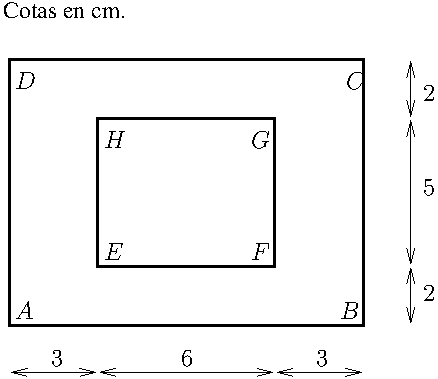
\includegraphics[width=0.35\textwidth]{ej1}
\end{center}

Se pide cargar los siguientes ficheros:

\begin{enumerate}
	\item Fichero de entrada de datos de feap
	\item Contornos de temperatura
	\item Contornos de flujo horizontal
\end{enumerate}

{\em NOTAS:}
\begin{itemize}
\item La malla estar� formada por elementos cuadrados de lado $0.2$ cm
\item En los puntos singulares en los que hay una condici�n de flujo y
temperatura impuestos de forma simult�nea, se considerar� la condici�n de
temperatura impuesta.
\item En el v�rtice $D$ la temperatura a considerar es $180$ $^{\circ}$K
\end{itemize}

\end{document}
